\documentclass{article}
\usepackage[utf8]{inputenc}
\usepackage{graphicx}
\usepackage{booktabs}
\usepackage{float}
\graphicspath{ {./fold_0/} }
\graphicspath{ {./fold_1/} }
\graphicspath{ {./fold_2/} }
\graphicspath{ {./fold_3/} }
\graphicspath{ {./fold_4/} }
\title{Results: bert-base-uncased-lr-[0.0005|0.00001|0.000001]}
\author{Nadia Sheikh}
\date{2022-06-26}
\begin{document}
\maketitle
\section{Configurations}
\subsection{Run Configuration}
\begin{tabular}{ll}
\toprule
{} &                                                  0 \\
\midrule
run\_identifier               &     bert-base-uncased-lr-[0.0005|0.00001|0.000001] \\
max\_epochs                   &                                                  3 \\
loss\_functions               &                                 cross-entropy-loss \\
learning\_rates               &                         0.00005, 0.00001, 0.000005 \\
batch\_sizes                  &                                                  1 \\
optimizers                   &                                               adam \\
llm\_name                     &                                  bert-base-uncased \\
hidden\_dropout\_prob          &                                                0.1 \\
attention\_probs\_dropout\_prob &                                                0.1 \\
pooling\_strategy             &                                               mean \\
config\_file\_path             &  /home/nadia/Documents/CLaC-Lab/ctre/cnc-task-3... \\
\bottomrule
\end{tabular}

\subsection{Data Configuration}
\begin{tabular}{ll}
\toprule
{} &                                                  0 \\
\midrule
data\_utility\_cls        &                                      cnc\_utilities \\
dataset\_cls             &                                   CNCTask3aDataset \\
nos\_of\_folds            &                                                  5 \\
trn\_data\_path           &  /home/nadia/Documents/CLaC-Lab/ctre/cnc-task-3... \\
tst\_data\_path           &  /home/nadia/Documents/CLaC-Lab/ctre/cnc-task-3... \\
base\_output\_folder\_path &  /home/nadia/Documents/CLaC-Lab/ctre/cnc-task-3... \\
config\_file\_path        &  //home/nadia/Documents/CLaC-Lab/ctre/cnc-task-... \\
\bottomrule
\end{tabular}

\subsection{Preprocessing Configuration}
\begin{tabular}{ll}
\toprule
{} &                                                  0 \\
\midrule
collate\_fn\_name   &                                       LLMCollateFn \\
llm\_name          &                                  bert-base-uncased \\
connl\_folder\_path &  /home/nadia/Documents/CLaC-Lab/ctre/cnc-task-3... \\
max\_nos\_tokens    &                                                 84 \\
token\_sep         &                                               True \\
config\_file\_path  &  /home/nadia/Documents/CLaC-Lab/ctre/cnc-task-3... \\
\bottomrule
\end{tabular}

\section{Hyperparameters}
\subsection{hparam\_config\_id\_0}
\begin{tabular}{ll}
\toprule
{} &                   0 \\
\midrule
loss\_function                &  cross-entropy-loss \\
learning\_rate                &             0.00005 \\
batch\_size                   &                   1 \\
optimizer                    &                adam \\
hidden\_dropout\_prob          &                 0.1 \\
attention\_probs\_dropout\_prob &                 0.1 \\
pooling\_strategy             &                mean \\
\bottomrule
\end{tabular}

\subsection{hparam\_config\_id\_1}
\begin{tabular}{ll}
\toprule
{} &                   0 \\
\midrule
loss\_function                &  cross-entropy-loss \\
learning\_rate                &             0.00001 \\
batch\_size                   &                   1 \\
optimizer                    &                adam \\
hidden\_dropout\_prob          &                 0.1 \\
attention\_probs\_dropout\_prob &                 0.1 \\
pooling\_strategy             &                mean \\
\bottomrule
\end{tabular}

\subsection{hparam\_config\_id\_2}
\begin{tabular}{ll}
\toprule
{} &                   0 \\
\midrule
loss\_function                &  cross-entropy-loss \\
learning\_rate                &            0.000005 \\
batch\_size                   &                   1 \\
optimizer                    &                adam \\
hidden\_dropout\_prob          &                 0.1 \\
attention\_probs\_dropout\_prob &                 0.1 \\
pooling\_strategy             &                mean \\
\bottomrule
\end{tabular}

\section{fold\_0}
\subsection{train\_loss}
\begin{tabular}{lrrr}
\toprule
{} &   ep 0 &   ep 1 &   ep 2 \\
\midrule
hp\_0 &  0.739 &  0.743 &  0.518 \\
hp\_1 &  0.727 &  0.676 &  0.441 \\
hp\_2 &  0.709 &  0.689 &  0.586 \\
\bottomrule
\end{tabular}

\begin{figure}[H]
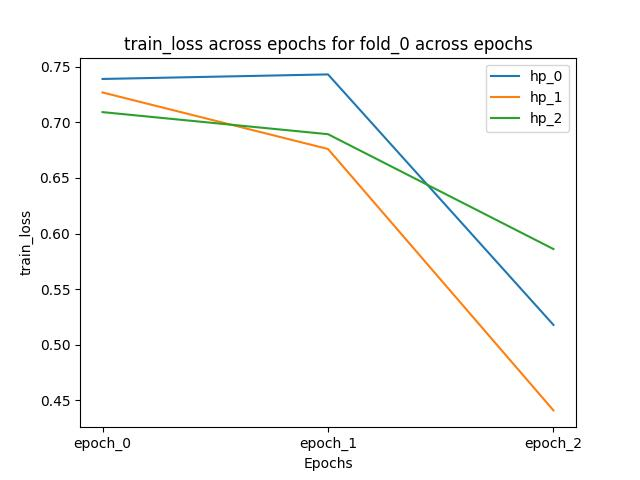
\includegraphics[scale = 0.75]{fold_0/train_loss}
\end{figure}
\subsection{test\_loss}
\begin{tabular}{lrrr}
\toprule
{} &   ep 0 &   ep 1 &   ep 2 \\
\midrule
hp\_0 &  0.683 &  0.722 &  0.604 \\
hp\_1 &  0.681 &  0.630 &  0.574 \\
hp\_2 &  0.687 &  0.658 &  0.593 \\
\bottomrule
\end{tabular}

\begin{figure}[H]
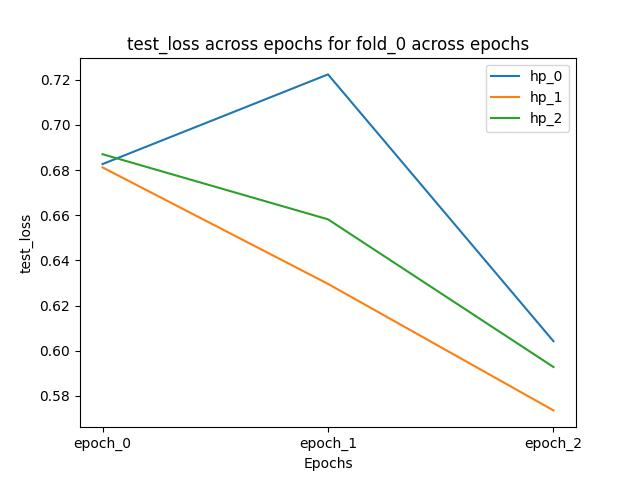
\includegraphics[scale = 0.75]{fold_0/test_loss}
\end{figure}
\subsection{accuracy\_score}
\begin{tabular}{lrrr}
\toprule
{} &  ep 0 &  ep 1 &  ep 2 \\
\midrule
hp\_0 &  0.54 &  0.48 &  0.76 \\
hp\_1 &  0.60 &  0.70 &  0.76 \\
hp\_2 &  0.62 &  0.68 &  0.74 \\
\bottomrule
\end{tabular}

\begin{figure}[H]
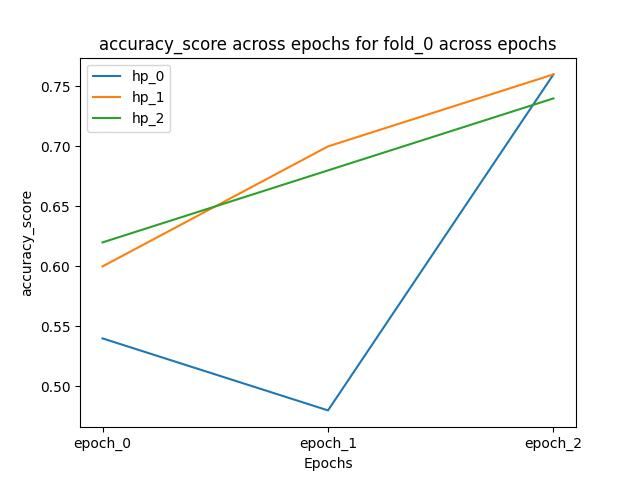
\includegraphics[scale = 0.75]{fold_0/accuracy_score}
\end{figure}
\subsection{f1\_score}
\begin{tabular}{lrrr}
\toprule
{} &   ep 0 &   ep 1 &   ep 2 \\
\midrule
hp\_0 &  0.667 &  0.649 &  0.760 \\
hp\_1 &  0.444 &  0.754 &  0.739 \\
hp\_2 &  0.678 &  0.733 &  0.755 \\
\bottomrule
\end{tabular}

\begin{figure}[H]
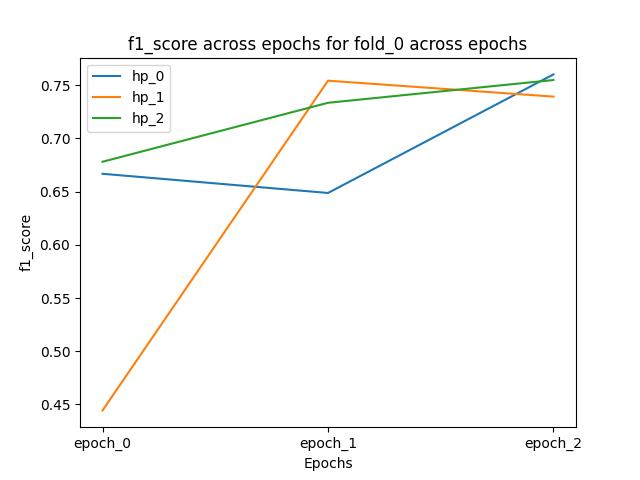
\includegraphics[scale = 0.75]{fold_0/f1_score}
\end{figure}
\subsection{precision\_score}
\begin{tabular}{lrrr}
\toprule
{} &   ep 0 &   ep 1 &   ep 2 \\
\midrule
hp\_0 &  0.511 &  0.480 &  0.731 \\
hp\_1 &  0.667 &  0.622 &  0.773 \\
hp\_2 &  0.571 &  0.611 &  0.690 \\
\bottomrule
\end{tabular}

\begin{figure}[H]
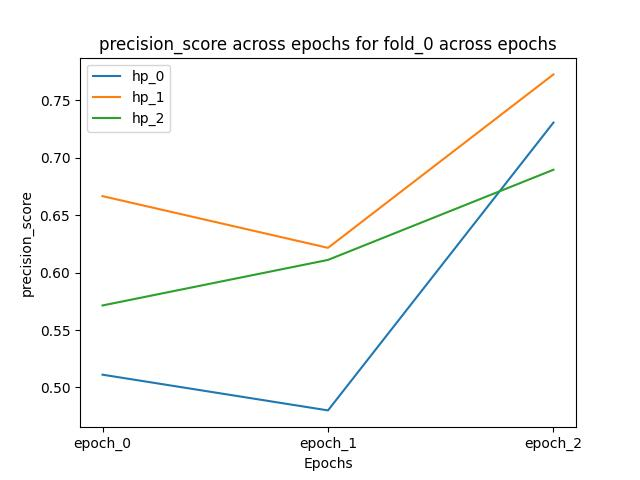
\includegraphics[scale = 0.75]{fold_0/precision_score}
\end{figure}
\subsection{matthews\_corrcoef}
\begin{tabular}{lrrr}
\toprule
{} &   ep 0 &   ep 1 &   ep 2 \\
\midrule
hp\_0 &  0.187 &  0.000 &  0.522 \\
hp\_1 &  0.210 &  0.478 &  0.519 \\
hp\_2 &  0.280 &  0.421 &  0.493 \\
\bottomrule
\end{tabular}

\begin{figure}[H]
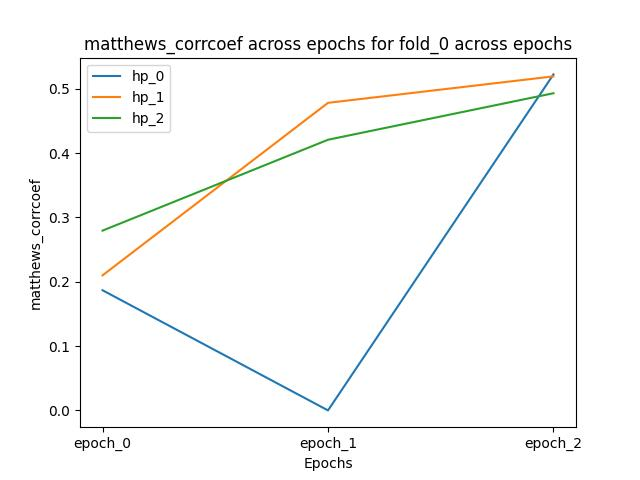
\includegraphics[scale = 0.75]{fold_0/matthews_corrcoef}
\end{figure}
\subsection{recall\_score}
\begin{tabular}{lrrr}
\toprule
{} &   ep 0 &   ep 1 &   ep 2 \\
\midrule
hp\_0 &  0.958 &  1.000 &  0.792 \\
hp\_1 &  0.333 &  0.958 &  0.708 \\
hp\_2 &  0.833 &  0.917 &  0.833 \\
\bottomrule
\end{tabular}

\begin{figure}[H]
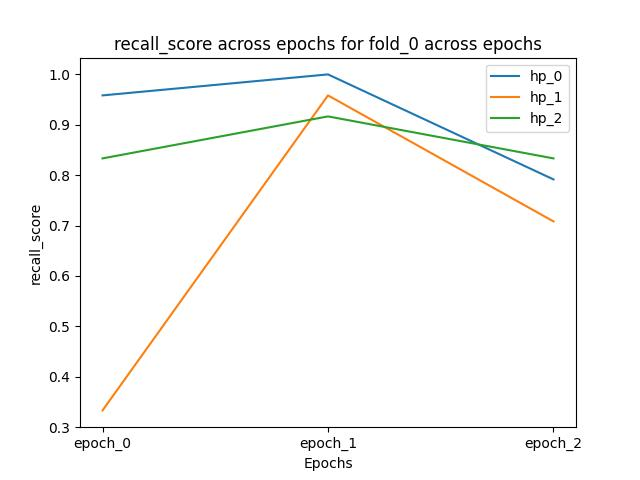
\includegraphics[scale = 0.75]{fold_0/recall_score}
\end{figure}
\section{fold\_1}
\subsection{train\_loss}
\begin{tabular}{lrrr}
\toprule
{} &   ep 0 &   ep 1 &   ep 2 \\
\midrule
hp\_0 &  0.732 &  0.710 &  0.423 \\
hp\_1 &  0.730 &  0.678 &  0.458 \\
hp\_2 &  0.714 &  0.687 &  0.600 \\
\bottomrule
\end{tabular}

\begin{figure}[H]
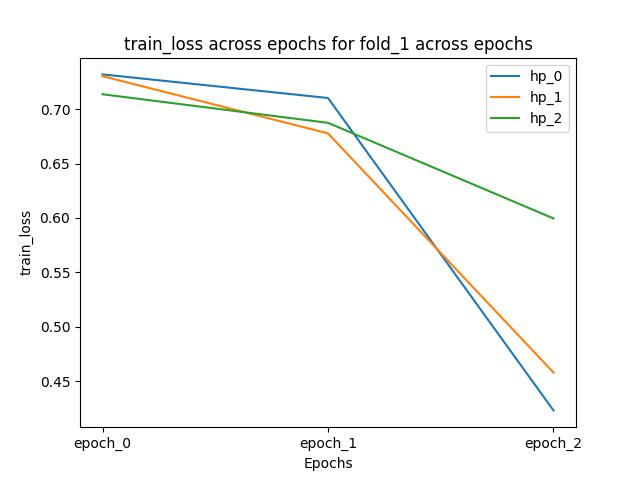
\includegraphics[scale = 0.75]{fold_1/train_loss}
\end{figure}
\subsection{test\_loss}
\begin{tabular}{lrrr}
\toprule
{} &   ep 0 &   ep 1 &   ep 2 \\
\midrule
hp\_0 &  0.689 &  0.639 &  0.633 \\
hp\_1 &  0.679 &  0.619 &  0.524 \\
hp\_2 &  0.700 &  0.671 &  0.633 \\
\bottomrule
\end{tabular}

\begin{figure}[H]
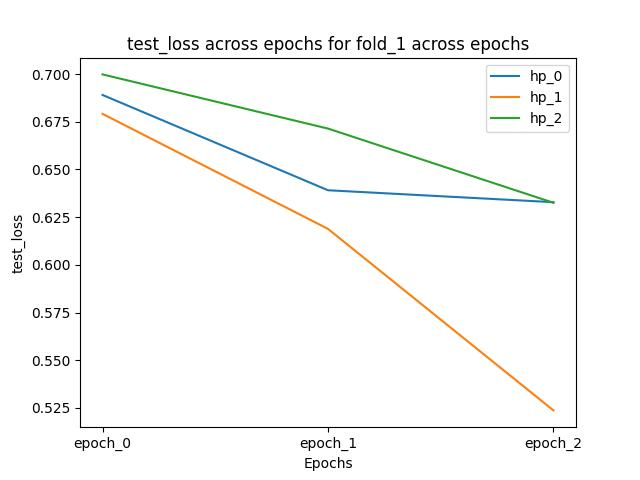
\includegraphics[scale = 0.75]{fold_1/test_loss}
\end{figure}
\subsection{accuracy\_score}
\begin{tabular}{lrrr}
\toprule
{} &  ep 0 &  ep 1 &  ep 2 \\
\midrule
hp\_0 &  0.54 &  0.58 &  0.70 \\
hp\_1 &  0.54 &  0.58 &  0.72 \\
hp\_2 &  0.54 &  0.56 &  0.72 \\
\bottomrule
\end{tabular}

\begin{figure}[H]
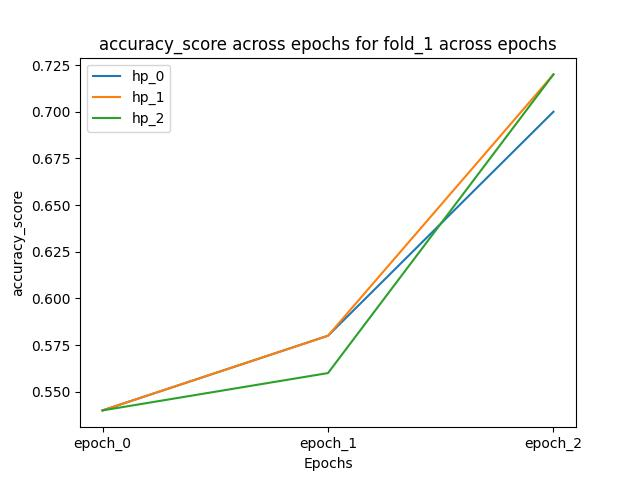
\includegraphics[scale = 0.75]{fold_1/accuracy_score}
\end{figure}
\subsection{f1\_score}
\begin{tabular}{lrrr}
\toprule
{} &   ep 0 &   ep 1 &   ep 2 \\
\midrule
hp\_0 &  0.701 &  0.667 &  0.769 \\
hp\_1 &  0.701 &  0.712 &  0.759 \\
hp\_2 &  0.685 &  0.703 &  0.781 \\
\bottomrule
\end{tabular}

\begin{figure}[H]
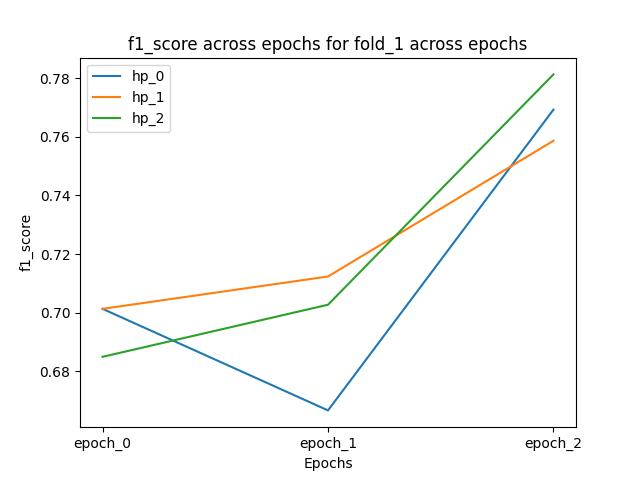
\includegraphics[scale = 0.75]{fold_1/f1_score}
\end{figure}
\subsection{precision\_score}
\begin{tabular}{lrrr}
\toprule
{} &   ep 0 &   ep 1 &   ep 2 \\
\midrule
hp\_0 &  0.540 &  0.583 &  0.658 \\
hp\_1 &  0.540 &  0.565 &  0.710 \\
hp\_2 &  0.543 &  0.553 &  0.676 \\
\bottomrule
\end{tabular}

\begin{figure}[H]
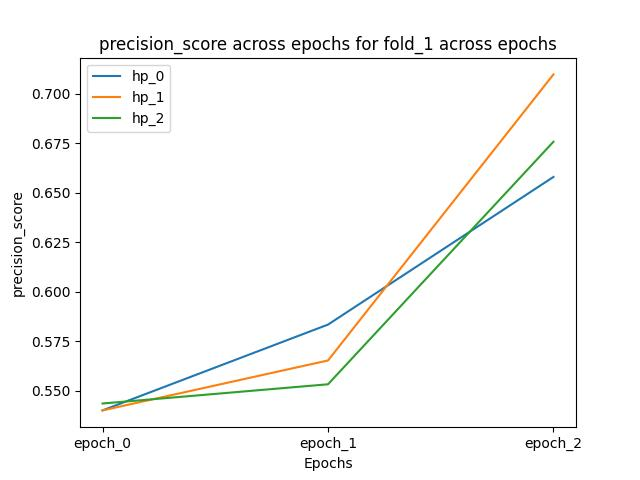
\includegraphics[scale = 0.75]{fold_1/precision_score}
\end{figure}
\subsection{matthews\_corrcoef}
\begin{tabular}{lrrr}
\toprule
{} &   ep 0 &   ep 1 &   ep 2 \\
\midrule
hp\_0 &  0.000 &  0.139 &  0.421 \\
hp\_1 &  0.000 &  0.172 &  0.435 \\
hp\_2 &  0.024 &  0.105 &  0.459 \\
\bottomrule
\end{tabular}

\begin{figure}[H]
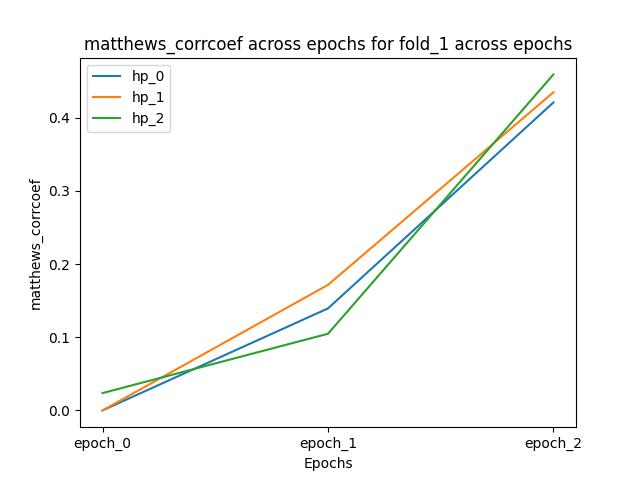
\includegraphics[scale = 0.75]{fold_1/matthews_corrcoef}
\end{figure}
\subsection{recall\_score}
\begin{tabular}{lrrr}
\toprule
{} &   ep 0 &   ep 1 &   ep 2 \\
\midrule
hp\_0 &  1.000 &  0.778 &  0.926 \\
hp\_1 &  1.000 &  0.963 &  0.815 \\
hp\_2 &  0.926 &  0.963 &  0.926 \\
\bottomrule
\end{tabular}

\begin{figure}[H]
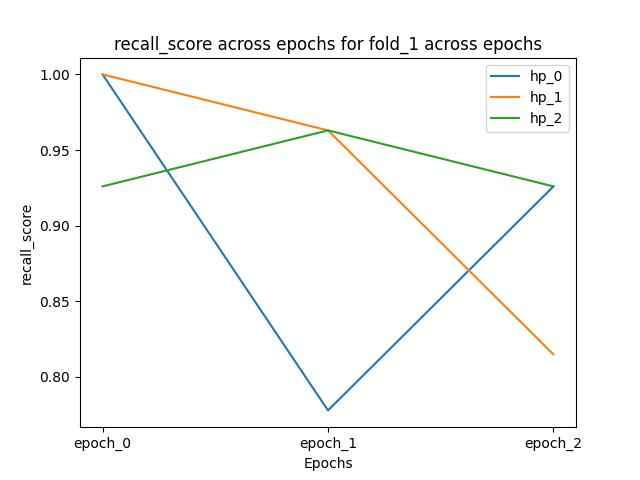
\includegraphics[scale = 0.75]{fold_1/recall_score}
\end{figure}
\section{fold\_2}
\subsection{train\_loss}
\begin{tabular}{lrrr}
\toprule
{} &   ep 0 &   ep 1 &   ep 2 \\
\midrule
hp\_0 &  0.728 &  0.699 &  0.412 \\
hp\_1 &  0.728 &  0.699 &  0.514 \\
hp\_2 &  0.723 &  0.697 &  0.576 \\
\bottomrule
\end{tabular}

\begin{figure}[H]
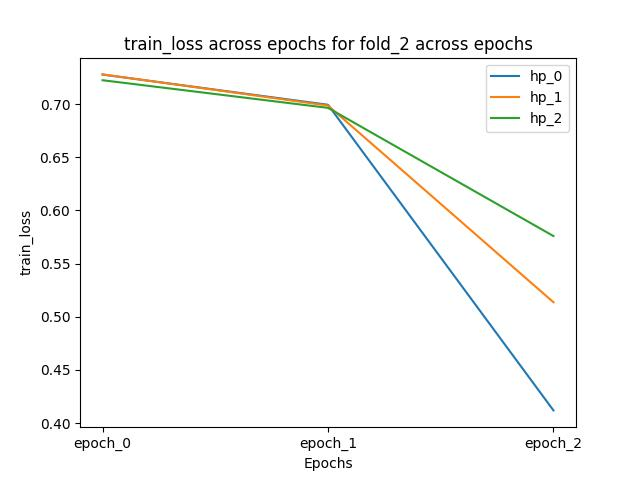
\includegraphics[scale = 0.75]{fold_2/train_loss}
\end{figure}
\subsection{test\_loss}
\begin{tabular}{lrrr}
\toprule
{} &   ep 0 &   ep 1 &   ep 2 \\
\midrule
hp\_0 &  0.698 &  0.714 &  1.057 \\
hp\_1 &  0.694 &  0.669 &  0.606 \\
hp\_2 &  0.683 &  0.691 &  0.699 \\
\bottomrule
\end{tabular}

\begin{figure}[H]
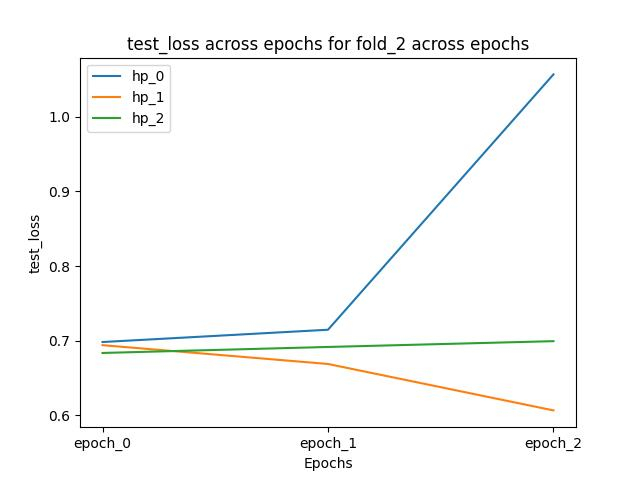
\includegraphics[scale = 0.75]{fold_2/test_loss}
\end{figure}
\subsection{accuracy\_score}
\begin{tabular}{lrrr}
\toprule
{} &  ep 0 &  ep 1 &  ep 2 \\
\midrule
hp\_0 &  0.46 &  0.66 &  0.62 \\
hp\_1 &  0.56 &  0.68 &  0.68 \\
hp\_2 &  0.58 &  0.52 &  0.60 \\
\bottomrule
\end{tabular}

\begin{figure}[H]
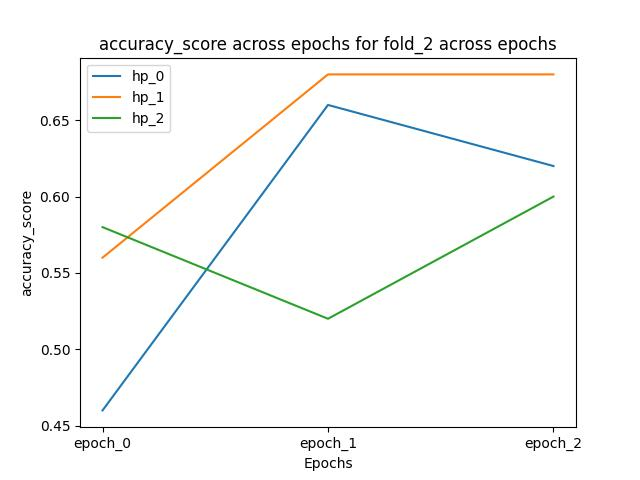
\includegraphics[scale = 0.75]{fold_2/accuracy_score}
\end{figure}
\subsection{f1\_score}
\begin{tabular}{lrrr}
\toprule
{} &   ep 0 &   ep 1 &   ep 2 \\
\midrule
hp\_0 &  0.609 &  0.564 &  0.667 \\
hp\_1 &  0.656 &  0.704 &  0.652 \\
hp\_2 &  0.087 &  0.613 &  0.655 \\
\bottomrule
\end{tabular}

\begin{figure}[H]
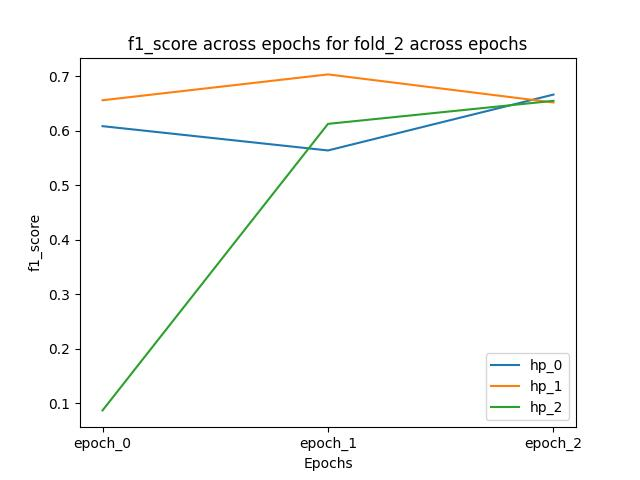
\includegraphics[scale = 0.75]{fold_2/f1_score}
\end{figure}
\subsection{precision\_score}
\begin{tabular}{lrrr}
\toprule
{} &   ep 0 &   ep 1 &   ep 2 \\
\midrule
hp\_0 &  0.438 &  0.611 &  0.528 \\
hp\_1 &  0.488 &  0.576 &  0.600 \\
hp\_2 &  0.500 &  0.463 &  0.514 \\
\bottomrule
\end{tabular}

\begin{figure}[H]
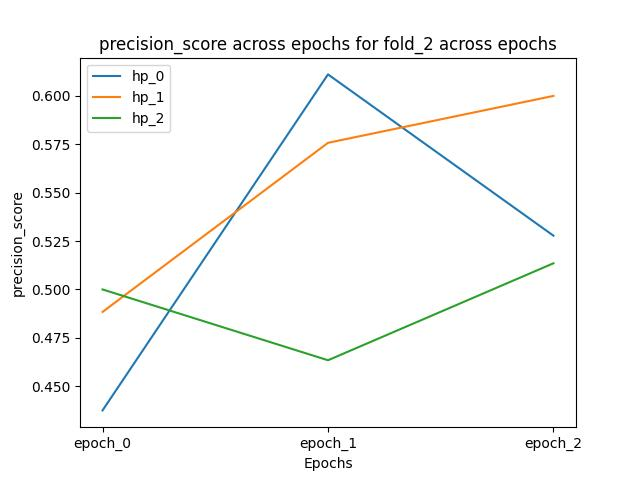
\includegraphics[scale = 0.75]{fold_2/precision_score}
\end{figure}
\subsection{matthews\_corrcoef}
\begin{tabular}{lrrr}
\toprule
{} &   ep 0 &   ep 1 &   ep 2 \\
\midrule
hp\_0 &  0.174 &  0.290 &  0.350 \\
hp\_1 &  0.343 &  0.440 &  0.365 \\
hp\_2 &  0.033 &  0.188 &  0.320 \\
\bottomrule
\end{tabular}

\begin{figure}[H]
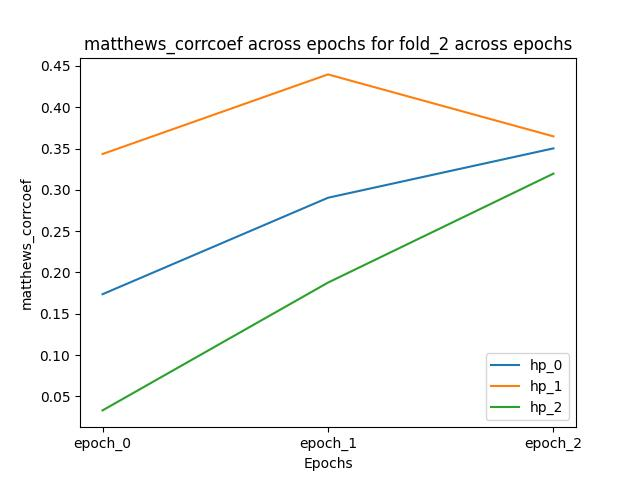
\includegraphics[scale = 0.75]{fold_2/matthews_corrcoef}
\end{figure}
\subsection{recall\_score}
\begin{tabular}{lrrr}
\toprule
{} &   ep 0 &   ep 1 &   ep 2 \\
\midrule
hp\_0 &  1.000 &  0.524 &  0.905 \\
hp\_1 &  1.000 &  0.905 &  0.714 \\
hp\_2 &  0.048 &  0.905 &  0.905 \\
\bottomrule
\end{tabular}

\begin{figure}[H]
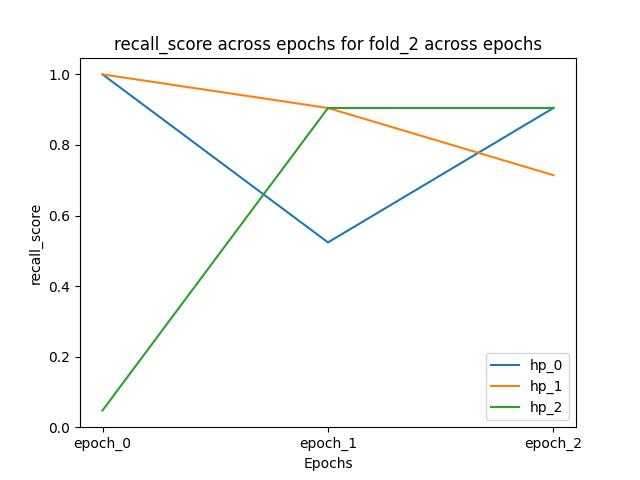
\includegraphics[scale = 0.75]{fold_2/recall_score}
\end{figure}
\section{fold\_3}
\subsection{train\_loss}
\begin{tabular}{lrrr}
\toprule
{} &   ep 0 &   ep 1 &   ep 2 \\
\midrule
hp\_0 &  0.752 &  0.693 &  0.424 \\
hp\_1 &  0.735 &  0.687 &  0.472 \\
hp\_2 &  0.713 &  0.678 &  0.542 \\
\bottomrule
\end{tabular}

\begin{figure}[H]
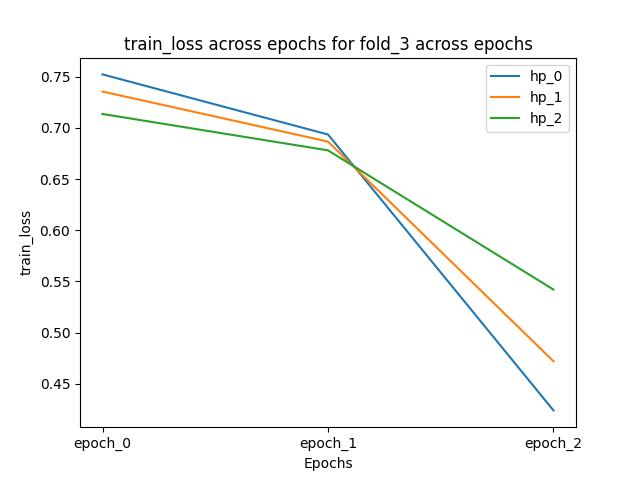
\includegraphics[scale = 0.75]{fold_3/train_loss}
\end{figure}
\subsection{test\_loss}
\begin{tabular}{lrrr}
\toprule
{} &   ep 0 &   ep 1 &   ep 2 \\
\midrule
hp\_0 &  0.730 &  0.675 &  0.536 \\
hp\_1 &  0.699 &  0.654 &  0.499 \\
hp\_2 &  0.754 &  0.693 &  0.631 \\
\bottomrule
\end{tabular}

\begin{figure}[H]
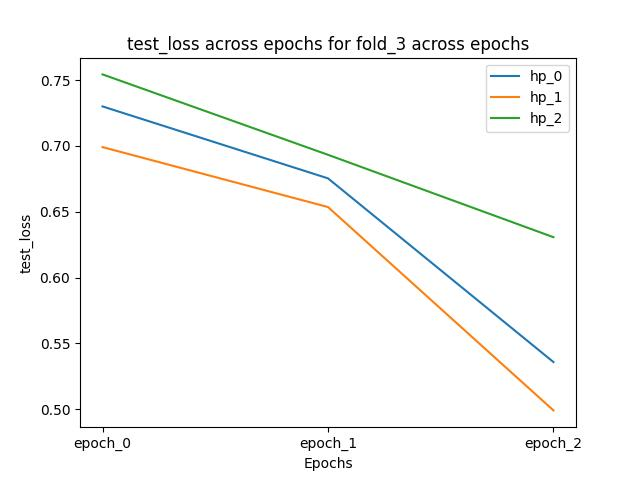
\includegraphics[scale = 0.75]{fold_3/test_loss}
\end{figure}
\subsection{accuracy\_score}
\begin{tabular}{lrrr}
\toprule
{} &  ep 0 &  ep 1 &  ep 2 \\
\midrule
hp\_0 &  0.46 &  0.62 &  0.72 \\
hp\_1 &  0.46 &  0.60 &  0.72 \\
hp\_2 &  0.42 &  0.48 &  0.62 \\
\bottomrule
\end{tabular}

\begin{figure}[H]
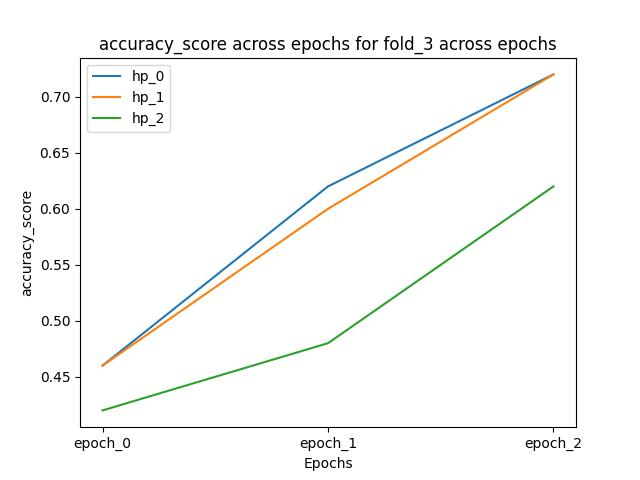
\includegraphics[scale = 0.75]{fold_3/accuracy_score}
\end{figure}
\subsection{f1\_score}
\begin{tabular}{lrrr}
\toprule
{} &   ep 0 &   ep 1 &   ep 2 \\
\midrule
hp\_0 &  0.000 &  0.513 &  0.741 \\
hp\_1 &  0.308 &  0.444 &  0.720 \\
hp\_2 &  0.000 &  0.278 &  0.578 \\
\bottomrule
\end{tabular}

\begin{figure}[H]
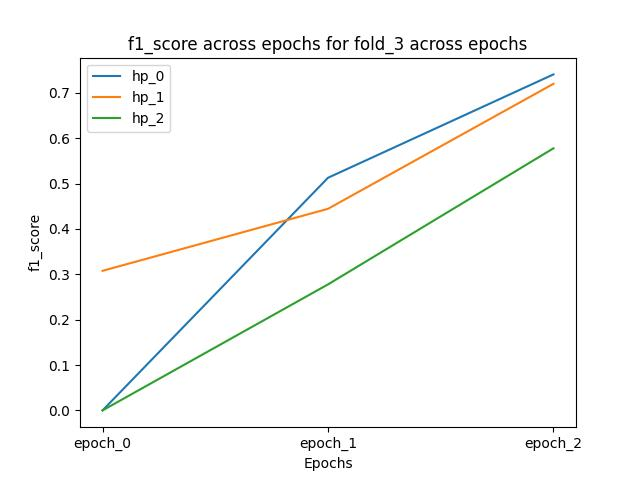
\includegraphics[scale = 0.75]{fold_3/f1_score}
\end{figure}
\subsection{precision\_score}
\begin{tabular}{lrrr}
\toprule
{} &  ep 0 &   ep 1 &   ep 2 \\
\midrule
hp\_0 &   0.0 &  0.833 &  0.741 \\
hp\_1 &   0.5 &  0.889 &  0.783 \\
hp\_2 &   0.0 &  0.556 &  0.722 \\
\bottomrule
\end{tabular}

\begin{figure}[H]
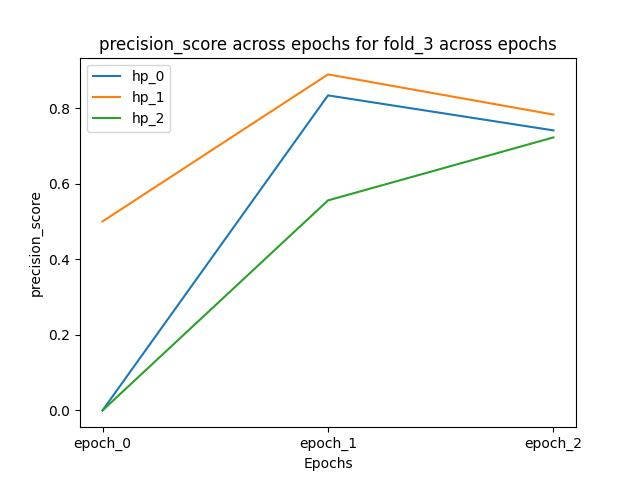
\includegraphics[scale = 0.75]{fold_3/precision_score}
\end{figure}
\subsection{matthews\_corrcoef}
\begin{tabular}{lrrr}
\toprule
{} &   ep 0 &   ep 1 &   ep 2 \\
\midrule
hp\_0 &  0.000 &  0.331 &  0.436 \\
hp\_1 & -0.045 &  0.328 &  0.449 \\
hp\_2 & -0.221 &  0.015 &  0.274 \\
\bottomrule
\end{tabular}

\begin{figure}[H]
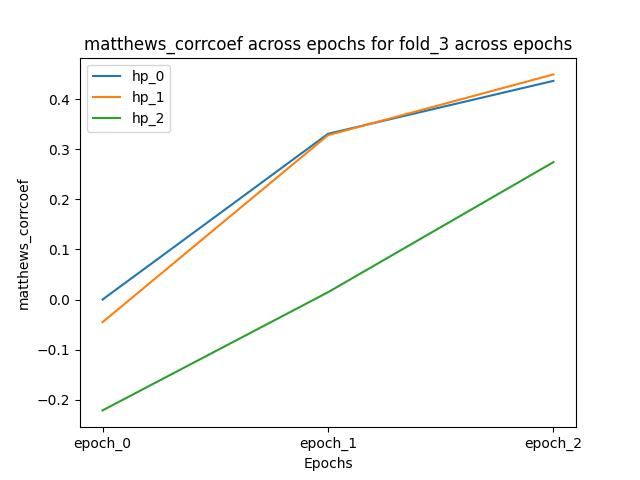
\includegraphics[scale = 0.75]{fold_3/matthews_corrcoef}
\end{figure}
\subsection{recall\_score}
\begin{tabular}{lrrr}
\toprule
{} &   ep 0 &   ep 1 &   ep 2 \\
\midrule
hp\_0 &  0.000 &  0.370 &  0.741 \\
hp\_1 &  0.222 &  0.296 &  0.667 \\
hp\_2 &  0.000 &  0.185 &  0.481 \\
\bottomrule
\end{tabular}

\begin{figure}[H]
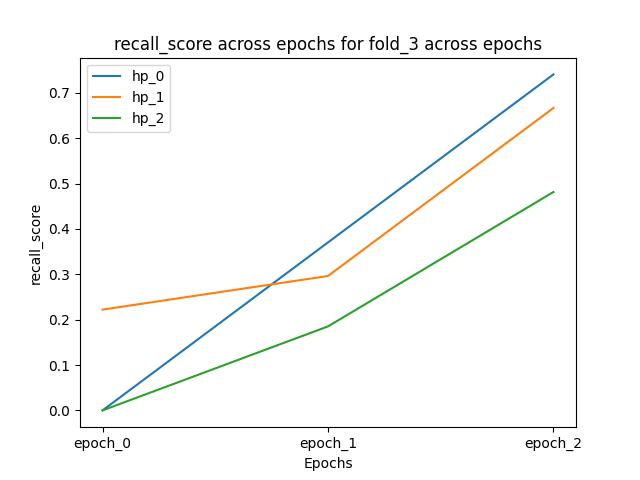
\includegraphics[scale = 0.75]{fold_3/recall_score}
\end{figure}
\section{fold\_4}
\subsection{train\_loss}
\begin{tabular}{lrrr}
\toprule
{} &   ep 0 &   ep 1 &   ep 2 \\
\midrule
hp\_0 &  0.751 &  0.738 &  0.689 \\
hp\_1 &  0.737 &  0.696 &  0.530 \\
hp\_2 &  0.720 &  0.698 &  0.609 \\
\bottomrule
\end{tabular}

\begin{figure}[H]
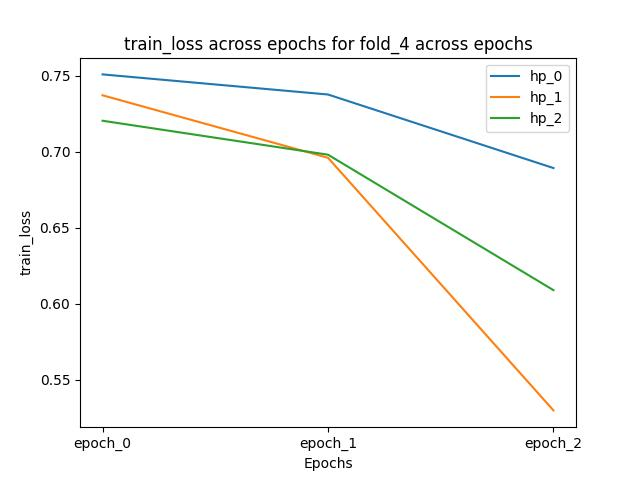
\includegraphics[scale = 0.75]{fold_4/train_loss}
\end{figure}
\subsection{test\_loss}
\begin{tabular}{lrrr}
\toprule
{} &   ep 0 &   ep 1 &   ep 2 \\
\midrule
hp\_0 &  0.695 &  0.693 &  0.561 \\
hp\_1 &  0.701 &  0.642 &  0.478 \\
hp\_2 &  0.686 &  0.655 &  0.591 \\
\bottomrule
\end{tabular}

\begin{figure}[H]
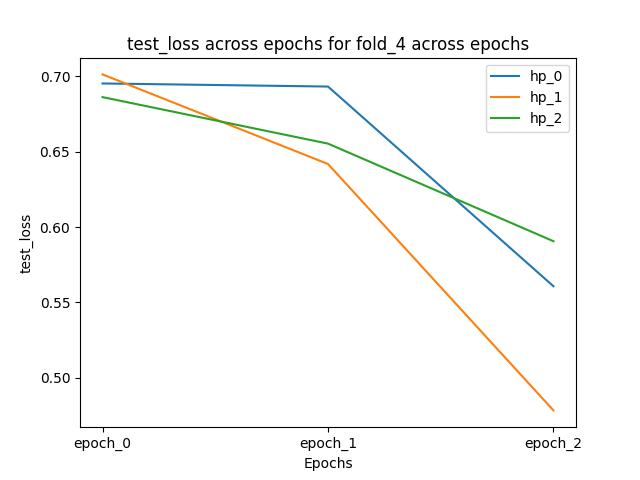
\includegraphics[scale = 0.75]{fold_4/test_loss}
\end{figure}
\subsection{accuracy\_score}
\begin{tabular}{lrrr}
\toprule
{} &  ep 0 &  ep 1 &  ep 2 \\
\midrule
hp\_0 &  0.48 &  0.46 &  0.74 \\
hp\_1 &  0.52 &  0.72 &  0.82 \\
hp\_2 &  0.52 &  0.60 &  0.68 \\
\bottomrule
\end{tabular}

\begin{figure}[H]
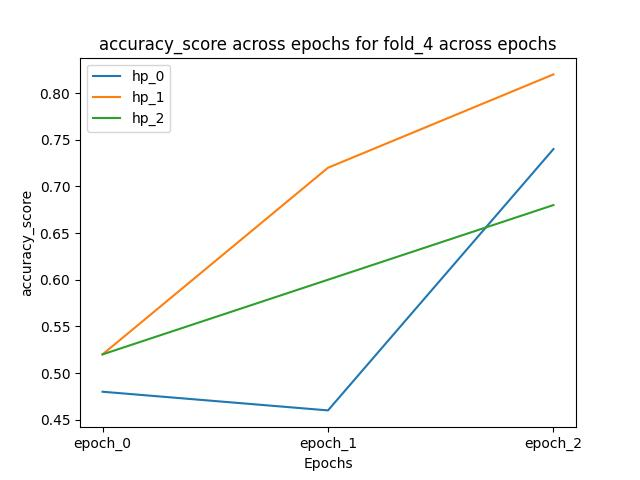
\includegraphics[scale = 0.75]{fold_4/accuracy_score}
\end{figure}
\subsection{f1\_score}
\begin{tabular}{lrrr}
\toprule
{} &   ep 0 &   ep 1 &   ep 2 \\
\midrule
hp\_0 &  0.581 &  0.630 &  0.723 \\
hp\_1 &  0.657 &  0.750 &  0.824 \\
hp\_2 &  0.478 &  0.643 &  0.714 \\
\bottomrule
\end{tabular}

\begin{figure}[H]
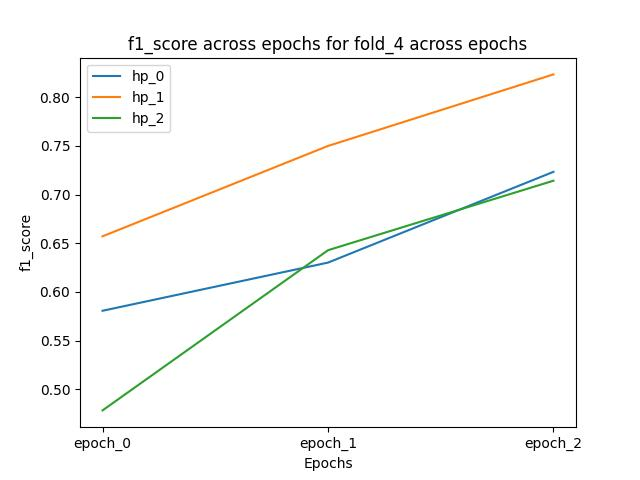
\includegraphics[scale = 0.75]{fold_4/f1_score}
\end{figure}
\subsection{precision\_score}
\begin{tabular}{lrrr}
\toprule
{} &   ep 0 &   ep 1 &   ep 2 \\
\midrule
hp\_0 &  0.462 &  0.460 &  0.708 \\
hp\_1 &  0.489 &  0.636 &  0.750 \\
hp\_2 &  0.478 &  0.545 &  0.606 \\
\bottomrule
\end{tabular}

\begin{figure}[H]
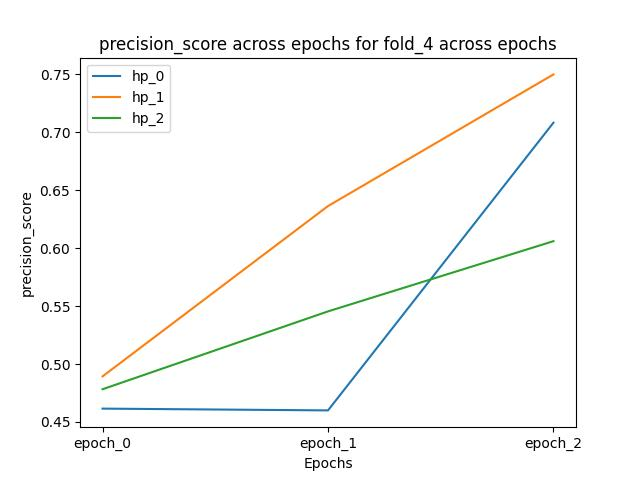
\includegraphics[scale = 0.75]{fold_4/precision_score}
\end{figure}
\subsection{matthews\_corrcoef}
\begin{tabular}{lrrr}
\toprule
{} &   ep 0 &   ep 1 &   ep 2 \\
\midrule
hp\_0 &  0.006 &  0.000 &  0.479 \\
hp\_1 &  0.233 &  0.493 &  0.656 \\
hp\_2 &  0.034 &  0.239 &  0.408 \\
\bottomrule
\end{tabular}

\begin{figure}[H]
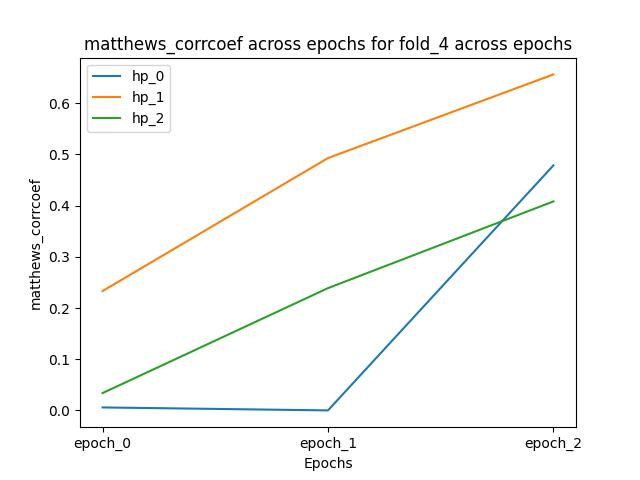
\includegraphics[scale = 0.75]{fold_4/matthews_corrcoef}
\end{figure}
\subsection{recall\_score}
\begin{tabular}{lrrr}
\toprule
{} &   ep 0 &   ep 1 &   ep 2 \\
\midrule
hp\_0 &  0.783 &  1.000 &  0.739 \\
hp\_1 &  1.000 &  0.913 &  0.913 \\
hp\_2 &  0.478 &  0.783 &  0.870 \\
\bottomrule
\end{tabular}

\begin{figure}[H]
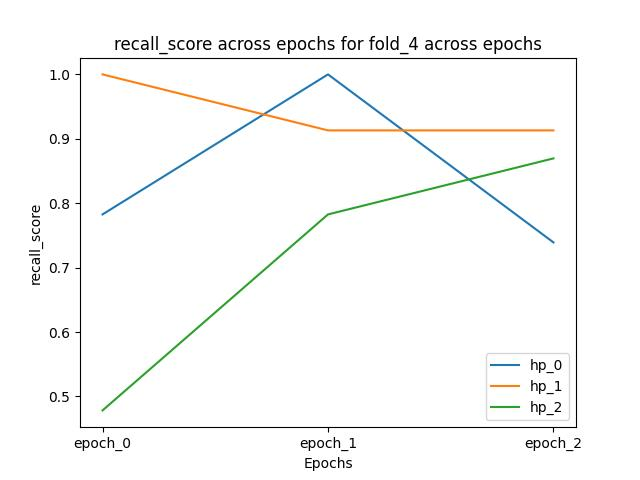
\includegraphics[scale = 0.75]{fold_4/recall_score}
\end{figure}
\end{document}
